\documentclass[11pt]{article}

\usepackage[utf8]{inputenc} % character encoding - you don't need to understand this

% Note that if you want to make a number sign, you need to type \#
% below are a bunch of useful packages, it doesn't cost anything to include them all so you might as well
\usepackage{amsmath}		            % lets you input equations in math mode
\usepackage{graphicx}		            % lets you include images
\usepackage{enumerate}		            % lets you make lists
\usepackage{subcaption}                 % if you want to use subcaptions
\usepackage[colorlinks=true]{hyperref}  % for making hyperlinks
\usepackage{hypcap}	                    % makes links refer to figures and not captions
\usepackage{relsize}		            % lets you use relative font sizes
\usepackage{caption}                    % lets you add captions
\usepackage{array}                      % lets you specify table column widths
\usepackage[margin=1in, paperwidth=8.5in, paperheight=11in]{geometry}
\usepackage{listings}
\usepackage{float}
\usepackage{tabularx}
\usepackage{textgreek}
\usepackage{amssymb}
\usepackage{amsthm}
\usepackage{placeins}
\usepackage{imakeidx}
\renewcommand{\qedsymbol}{$\blacksquare$}
\usepackage{blindtext}
\usepackage{csquotes}
\usepackage[style=numeric-comp,sorting=none]{biblatex}
% \usepackage{biblatex}
\addbibresource{thesis.bib}
\makeindex[columns=2, title=Alphabetical Index, 
options= -s example_style.ist, intoc]

% Note that if you want to make a number sign, you need to type \#
\hypersetup{
    colorlinks=true,
    linkcolor=blue,
    filecolor=magenta,
    urlcolor=cyan,
}

\lstdefinestyle{mystyle}{
  backgroundcolor=\color{backcolour},   commentstyle=\color{codegreen},
  keywordstyle=\color{magenta},
  numberstyle=\tiny\color{codegray},
  stringstyle=\color{codepurple},
  basicstyle=\ttfamily\footnotesize,
  breakatwhitespace=false,         
  breaklines=true,                 
  captionpos=b,                    
  keepspaces=true,                 
  numbers=left,                    
  numbersep=5pt,                  
  showspaces=false,                
  showstringspaces=false,
  showtabs=false,                  
  tabsize=2
}

\begin{document}
\title{Mixed Analog-Digital VLSI Mini-Project II: 4-Bit Shift Register}
\author{Qingmu Deng}
\maketitle % this line makes the title appear, along with today's date, automatically updated.

\section*{Project Links}

Project Github: \href{https://github.com/QingmuDeng/MADVLSI/tree/main/mini2}{https://github.com/QingmuDeng/MADVLSI/tree/main/mini2}

\noindent
Project zip file: \href{https://github.com/QingmuDeng/MADVLSI/blob/main/mini2/Deng-mini2.zip?raw=true}{https://github.com/QingmuDeng/MADVLSI/blob/main/mini2/Deng-mini2.zip?raw=true}
\section{Background}
    The D flip-flop design in this project is inspired by the thesis work by Sivilotti. [Sivilotti91] One important aspect of the D flip-flop operation is the ratio between the strength ratio of the pull up/down transistors and that of the pass transistors. Too strong of a pass transistor could potentially propagate the behaviors of downstream flip-flops upstreams and result in set/reset issues. The equation of merit is
    \begin{align}
        \frac{S_{Q_{pull}}}{S_{pass}} > \frac{(\phi-V_{Tn}-nV_A)}{2n(\phi-V_{Tn})V_A-n^2V_A^2}
    \end{align}
    where $\phi$ is the clock voltage, $V_{Tn}$ the threshold voltage of the transistors, $n$ the subthreshold slope factor, and $V_A$ the voltage at the drain of the pass transistor. Plotting the righthand side equation against the clock voltage, while assuming $V_A=V_{Tn}=0.52V$ and $n=1.4$, gives us Figure \ref{fig:sratio}.
    \begin{figure}[!ht]
        \centering
        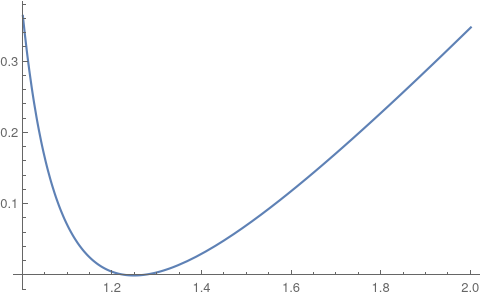
\includegraphics[width=.6\linewidth]{../img/sratio.png}
        \caption{Minimal ratio of the pull/pass transistor strength ratio.}
        \label{fig:sratio}
    \end{figure}
    The conclusion is that a ratio of 1 should work, as will be shown in the simulations of the next section. In actual D flip-flop design, we adopt the alternative schematic shown in Figure \ref{fig:alt} for better schematic and layout symmetry.
    \begin{figure}[!ht]
        \centering
        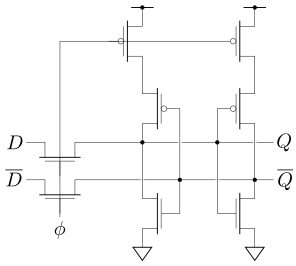
\includegraphics[width=.3\linewidth]{../img/altCSRLphilatch.png}
        \caption{Alternative CSRL Design to be used in the rest of the project.}
        \label{fig:alt}
    \end{figure}

\section{Schematic Capture and Simulation}
    To design a rising-edge triggered complementary set-reset logic D flip-flop, I joined two set-reset latches that are inverted version of one another. The layout driven schematic of this design is shown in Figure \ref{fig:dff}. The strength ratio of the pull up/down transistor to that of the pass transistor is chosen to be 1, because it not only provides a consistent transistor size for subsequent layout but has been proven to work in Figure \ref{fig:dff_s1}. Similar tests were performed with hierarchical schematics shown in Figure \ref{fig:dff_test}. 

    Next, I daisy-chained four D flip-flop together to form a 4-bit shift register as shown in Figure \ref{fig:shiftreg}. I also created the test harness in Figure \ref{fig:sreg_test} to validate the functionality of the shift register. The results in Figure \ref{fig:sreg_test_out} shows that the shift register is capable of shifting a bit through the entire device without glitches.
    \begin{figure}[!ht]
        \centering
        \begin{subfigure}{\linewidth}
            \centering
            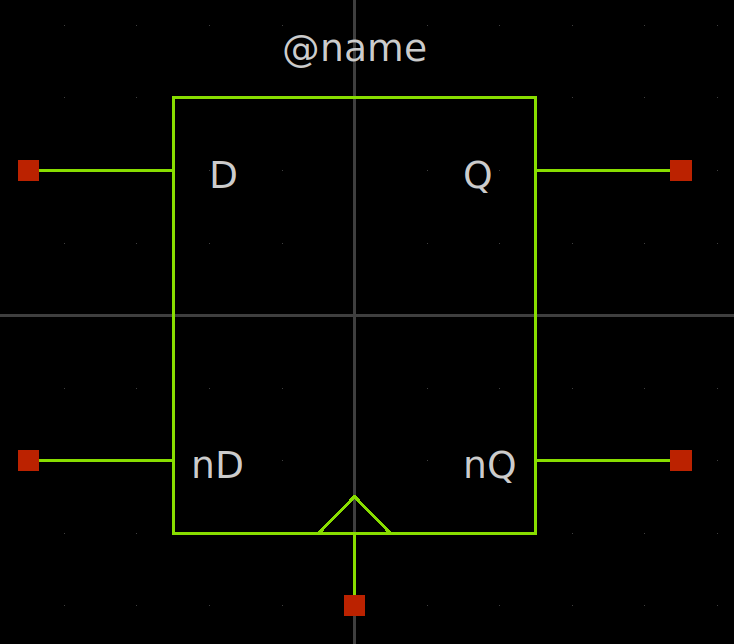
\includegraphics[width=0.2\linewidth]{../img/dff_sym.png}
            \caption{Rising-edge D flip-flop symbol created in Xschem.}
        \end{subfigure}\\
        \begin{subfigure}{0.8\linewidth}
            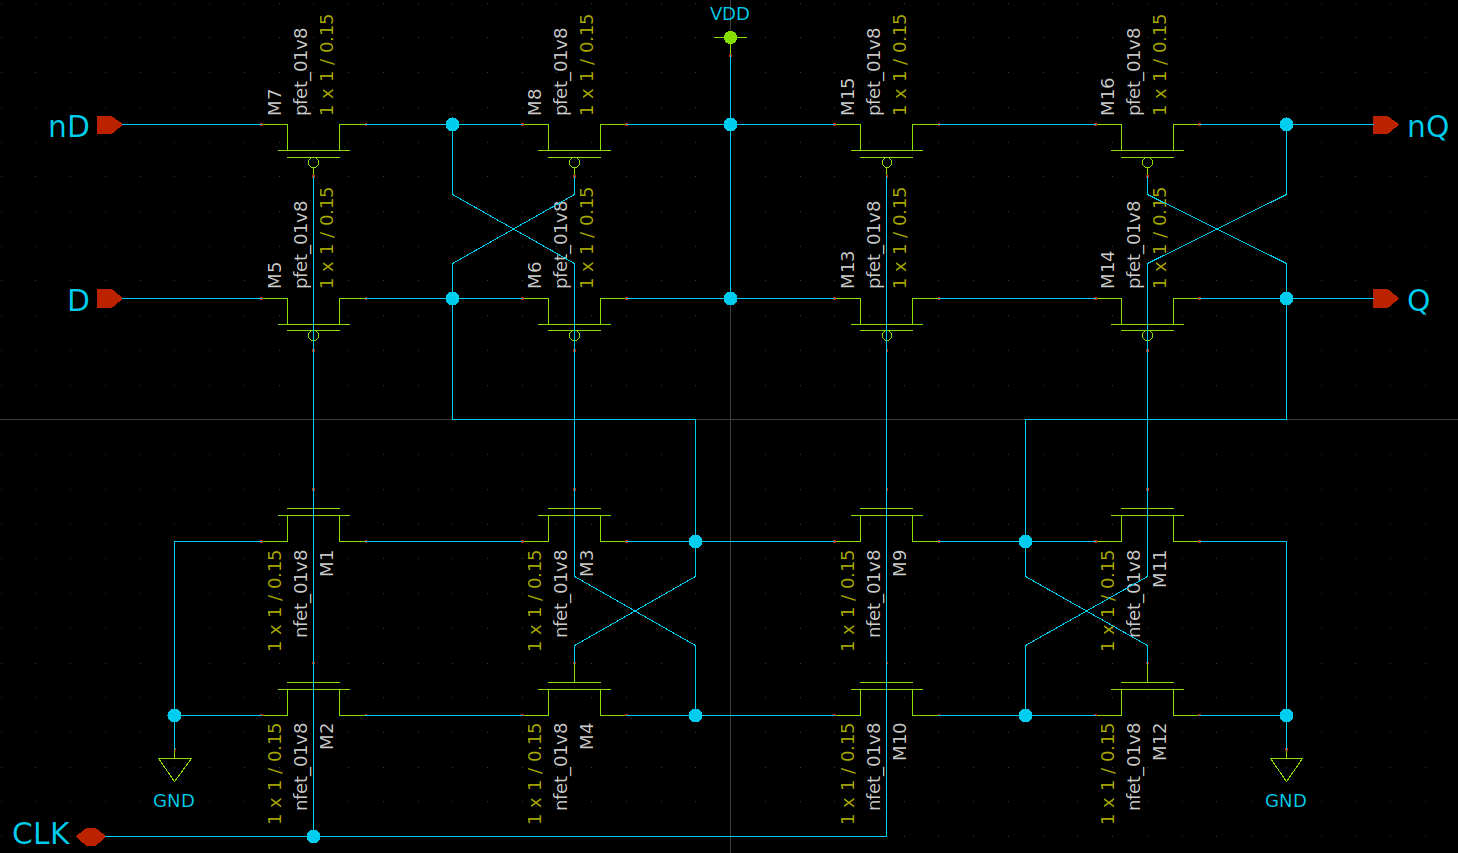
\includegraphics[width=\linewidth]{../img/dff_sch.png}
            \caption{D flip-flop layout-driven schematic created in Xschem.}
        \end{subfigure}
        \caption{D flip-flop design in Xschem.}
        \label{fig:dff}
    \end{figure}
    \begin{figure}[!ht]
        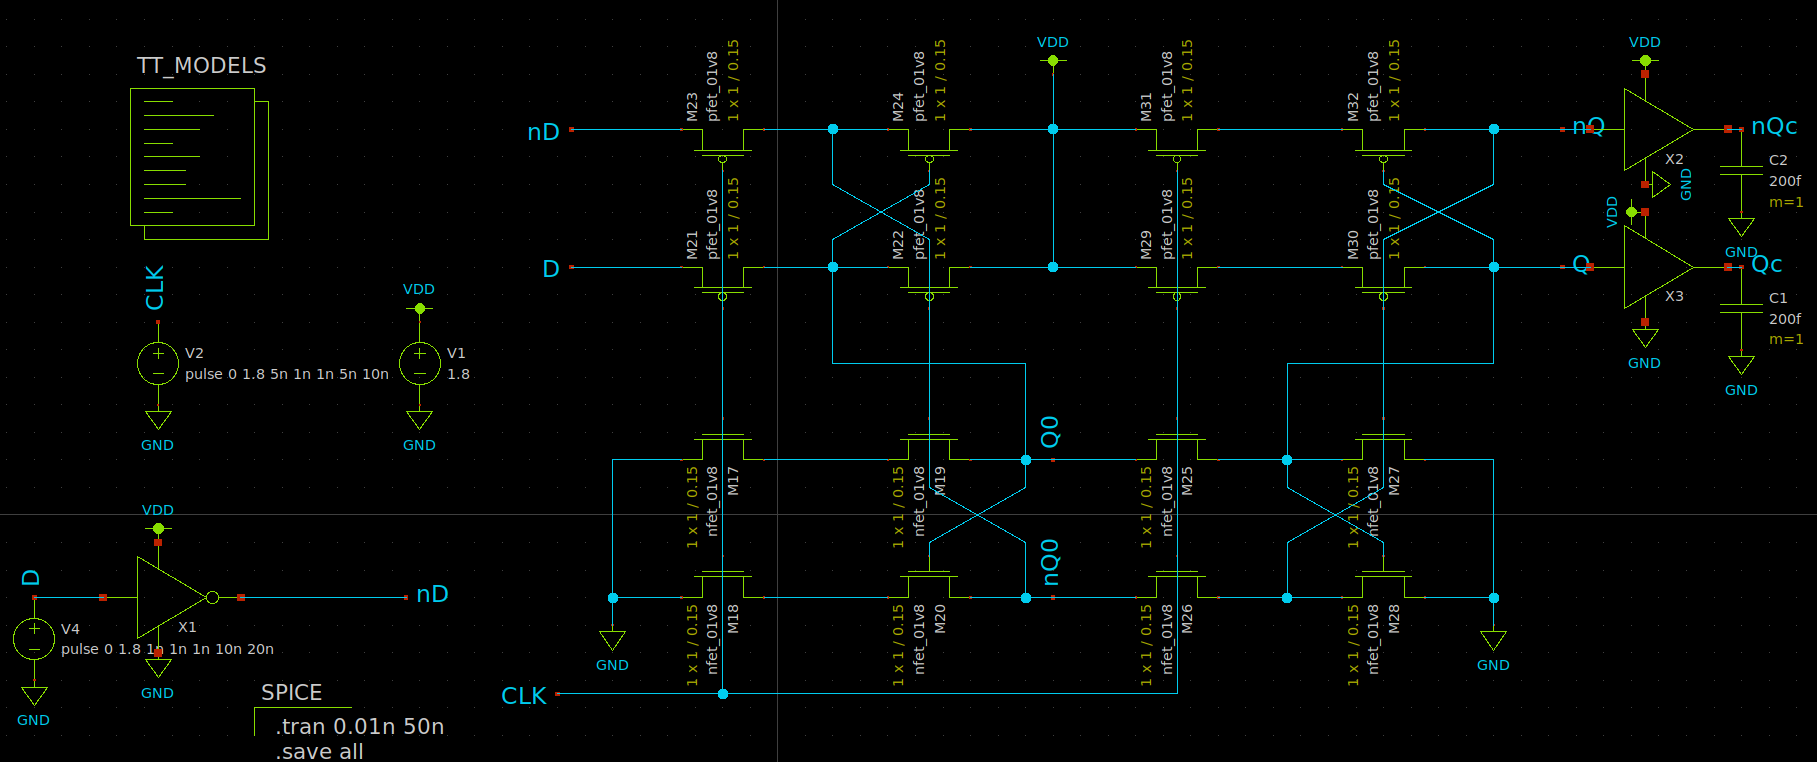
\includegraphics[width=\linewidth]{../img/dff_stest_harness.png}
        \caption{D flip-flop strength ratio test harness created in Xschem.}
        \label{fig:dff_stest}
    \end{figure}
    \begin{figure}[!ht]
        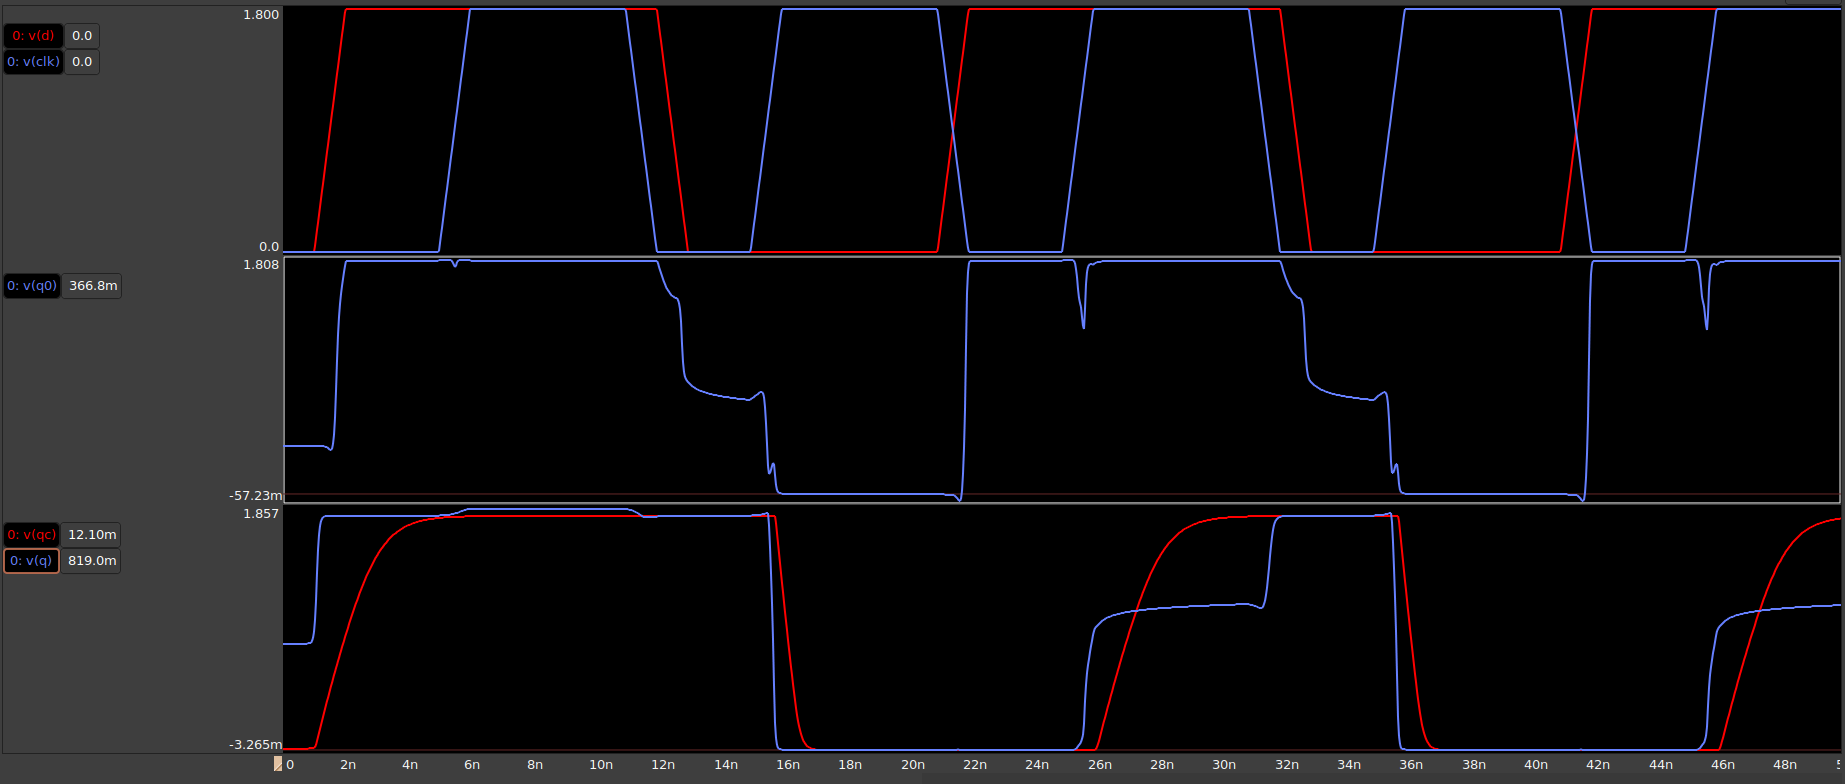
\includegraphics[width=\linewidth]{../img/S_1}
        \caption{Pull up/down-to-Pass ratio test result for a ratio of 1.}
        \label{fig:dff_s1}
    \end{figure}
    \begin{figure}[!ht]
        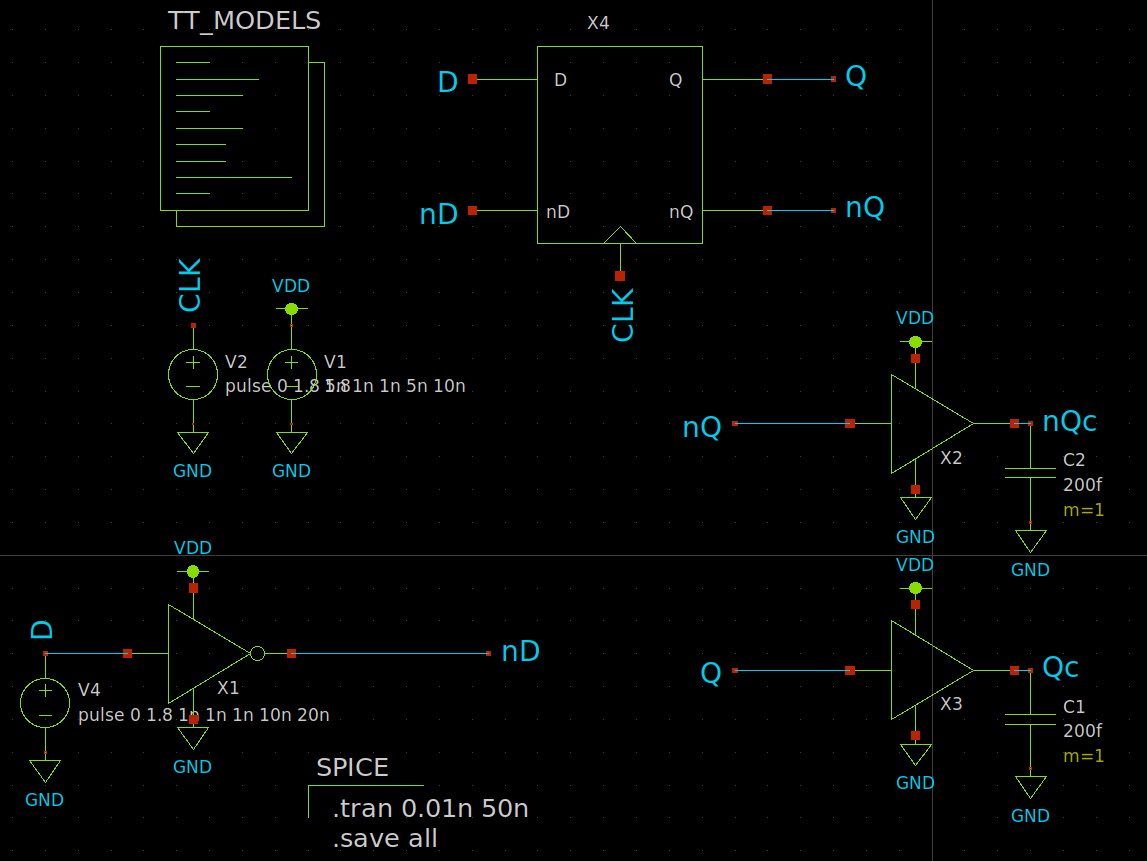
\includegraphics[width=\linewidth]{../img/dff_test_harness.png}
        \caption{D flip-flop function test harness created in Xschem.}
        \label{fig:dff_test}
    \end{figure}
    \begin{figure}[!ht]
        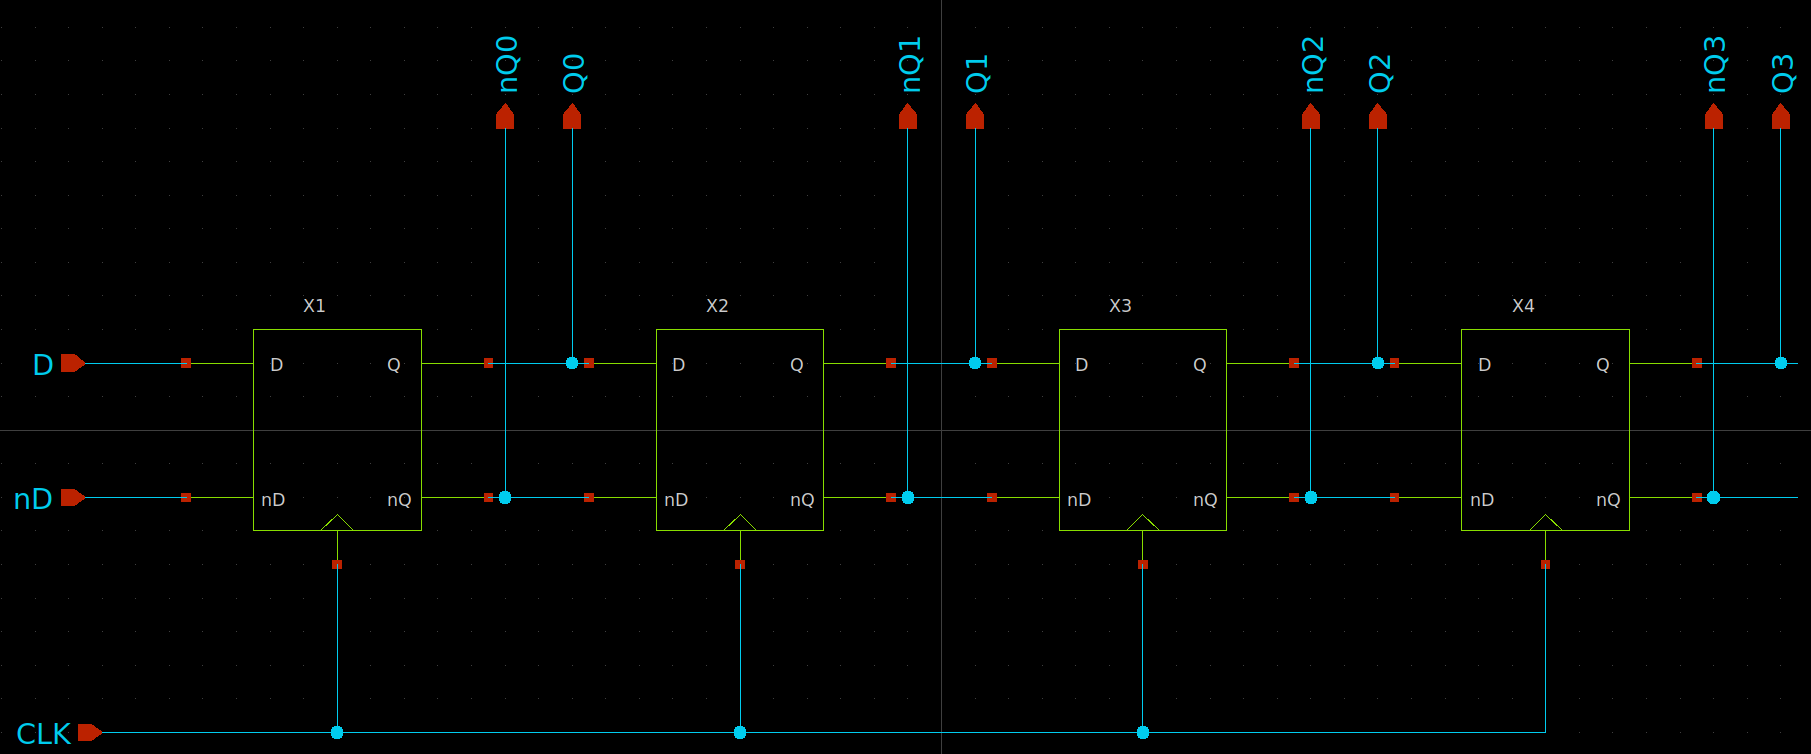
\includegraphics[width=\linewidth]{../img/sreg_sch.png}
        \caption{NAND2 schematic created in Xschem.}
        \label{fig:shiftreg}
    \end{figure}
    \begin{figure}[!ht]
        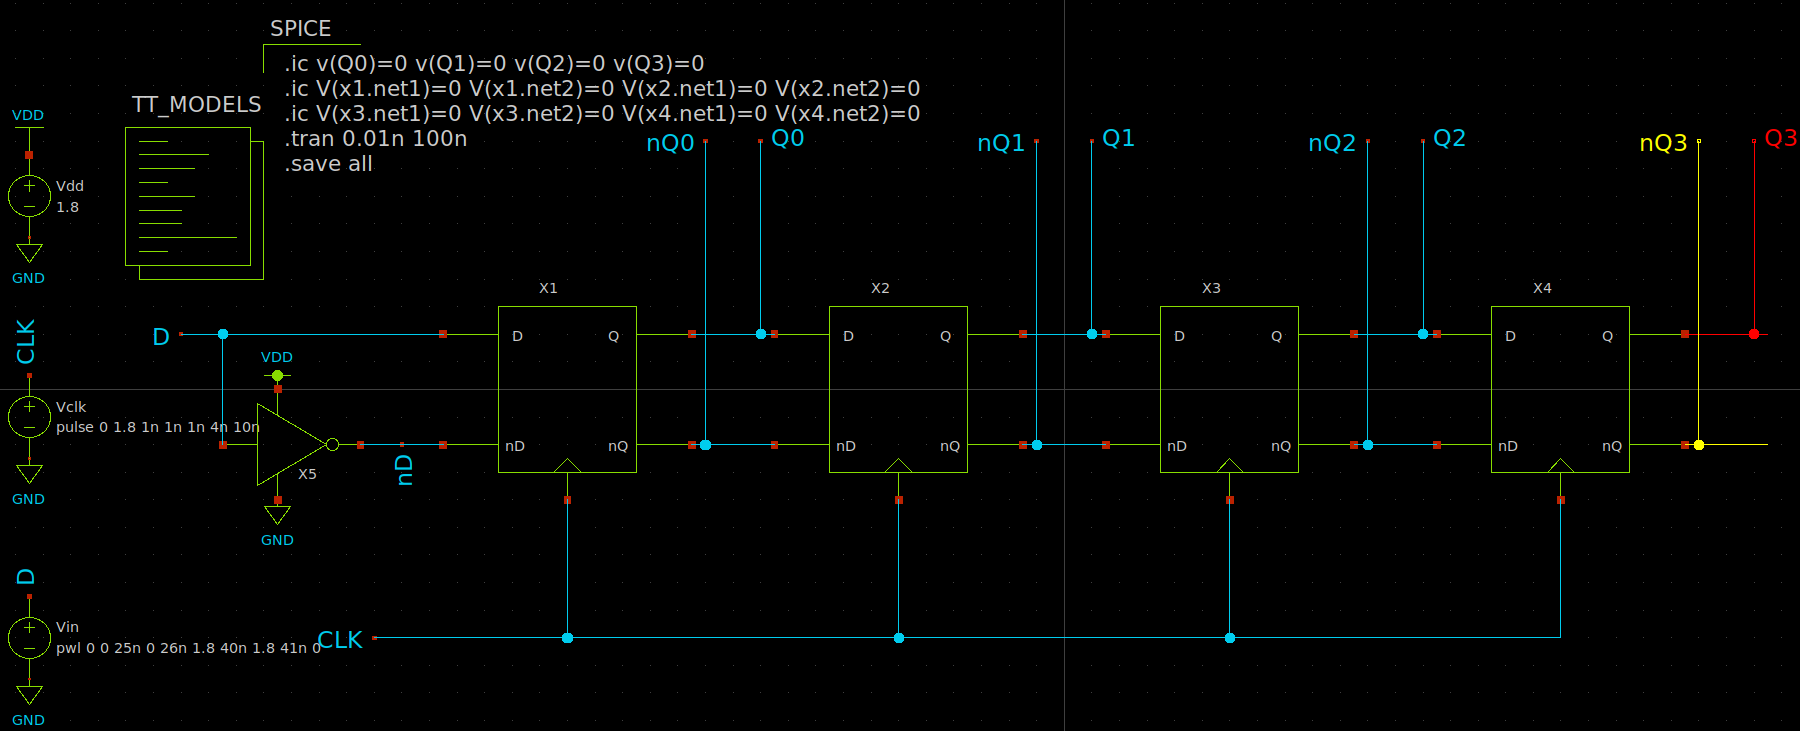
\includegraphics[width=\linewidth]{../img/sreg_test_hardness.png}
        \caption{D flip-flop function test harness created in Xschem.}
        \label{fig:sreg_test}
    \end{figure}
    \begin{figure}[!ht]
        \centering
        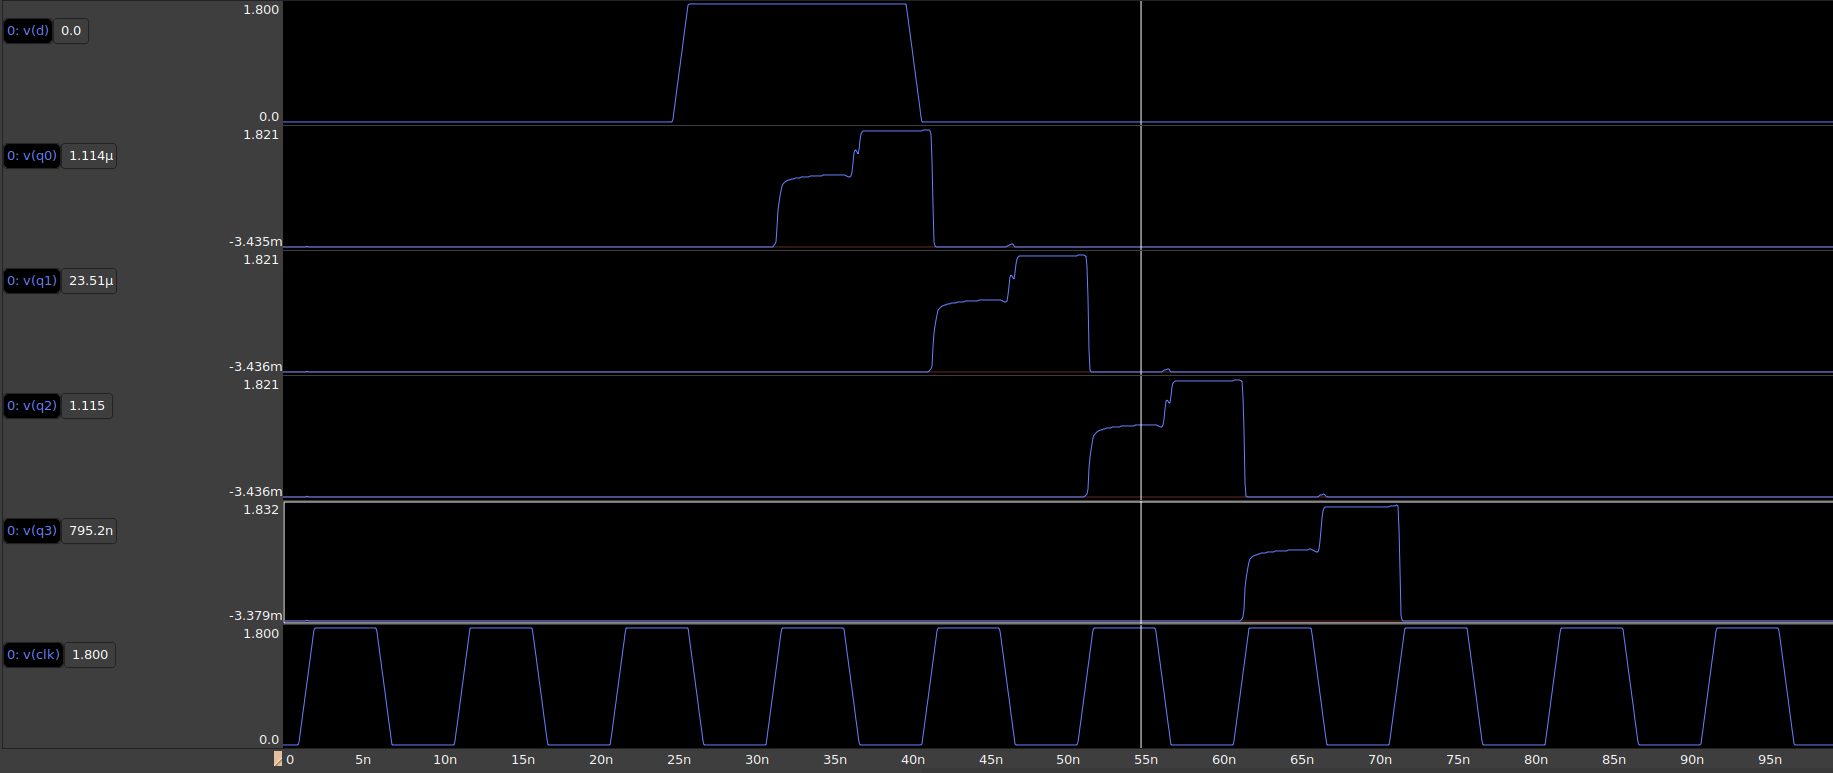
\includegraphics[width=1.2\linewidth, angle=90]{../img/sreg_test.png}
        \caption{D flip-flop function test harness created in Xschem.}
        \label{fig:sreg_test_out}
    \end{figure}
    

\FloatBarrier
\section{Layout Design}
    To begin with, I laid out my D flip-flop design in \text{Magic}. As shown in Figure \ref{fig:dffmag}, a \textbf{standalone} cell has the following dimensions.
    \begin{itemize}
        \item Width: 3.40 $\mu$m
        \item Height: 9.90 $\mu$m
    \end{itemize} 
    However, the standalone cell include extra \textit{nwell} region necessary for meeting the DRC at the cell level. When abutting adjecent cells together to form a shift register, individual D flip-flop are allowed to overlap, resulting in the following \textbf{effective} dimensions.
    \begin{itemize}
        \item Width: 3.15 $\mu$m
        \item Height: 9.90 $\mu$m
    \end{itemize} 
    Figure \ref{fig:sregmag} shows such a design. The overall size of the shift register without inverter is 
    \begin{itemize}
        \item Width: 12.85 $\mu$m
        \item Height: 9.90 $\mu$m
    \end{itemize}
    To allow for the accomodation of the shift register design for digital data whose inverse is not readily availble, Figure \ref{fig:sregmag_inv} shows a design with inverter staged before the first D flip-flop to generate the inverse signal for input. The overall size of the design with an inverter is 
    \begin{itemize}
        \item Width: 14.35 $\mu$m
        \item Height: 9.90 $\mu$m 
    \end{itemize}.
    There are no design rule violations.

    \begin{figure}[!ht]
        \centering
        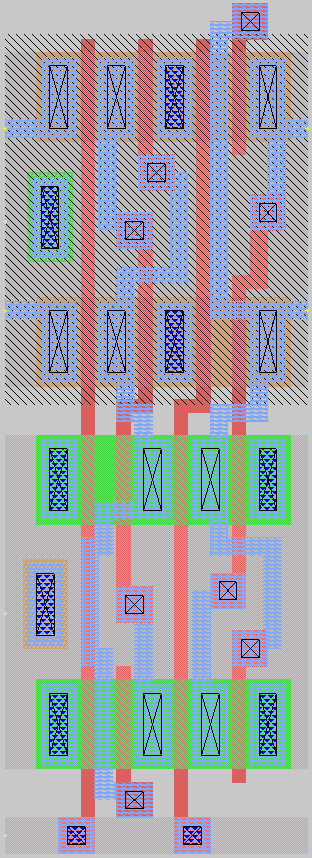
\includegraphics[width=0.3\linewidth]{../img/dff_mag.png}
        \caption{\textit{Magic} layout of the D flip-flop.}
        \label{fig:dffmag}
    \end{figure}
    \begin{figure}[!ht]
        \centering
        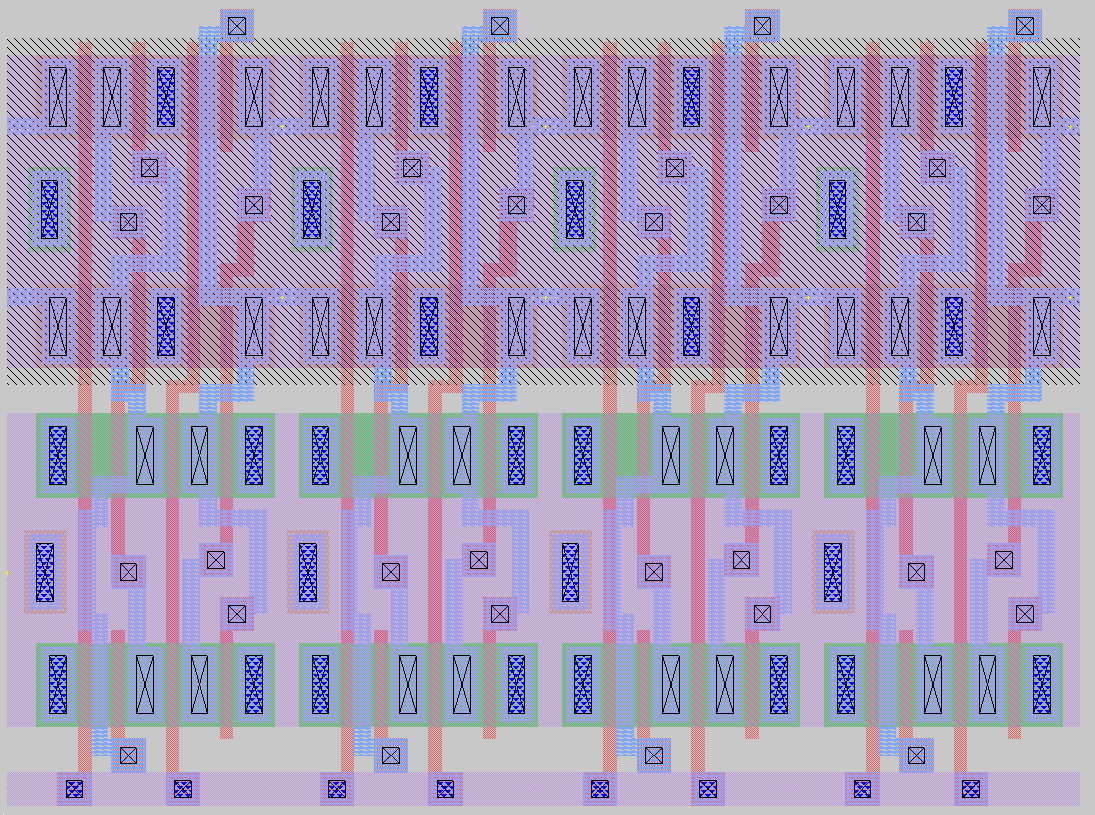
\includegraphics[width=0.8\linewidth]{../img/shiftreg_4.png}
        \caption{\textit{Magic} layout of the shift register by abutting four D flip-flops.}
        \label{fig:sregmag}
    \end{figure}
    \begin{figure}[!ht]
        \centering
        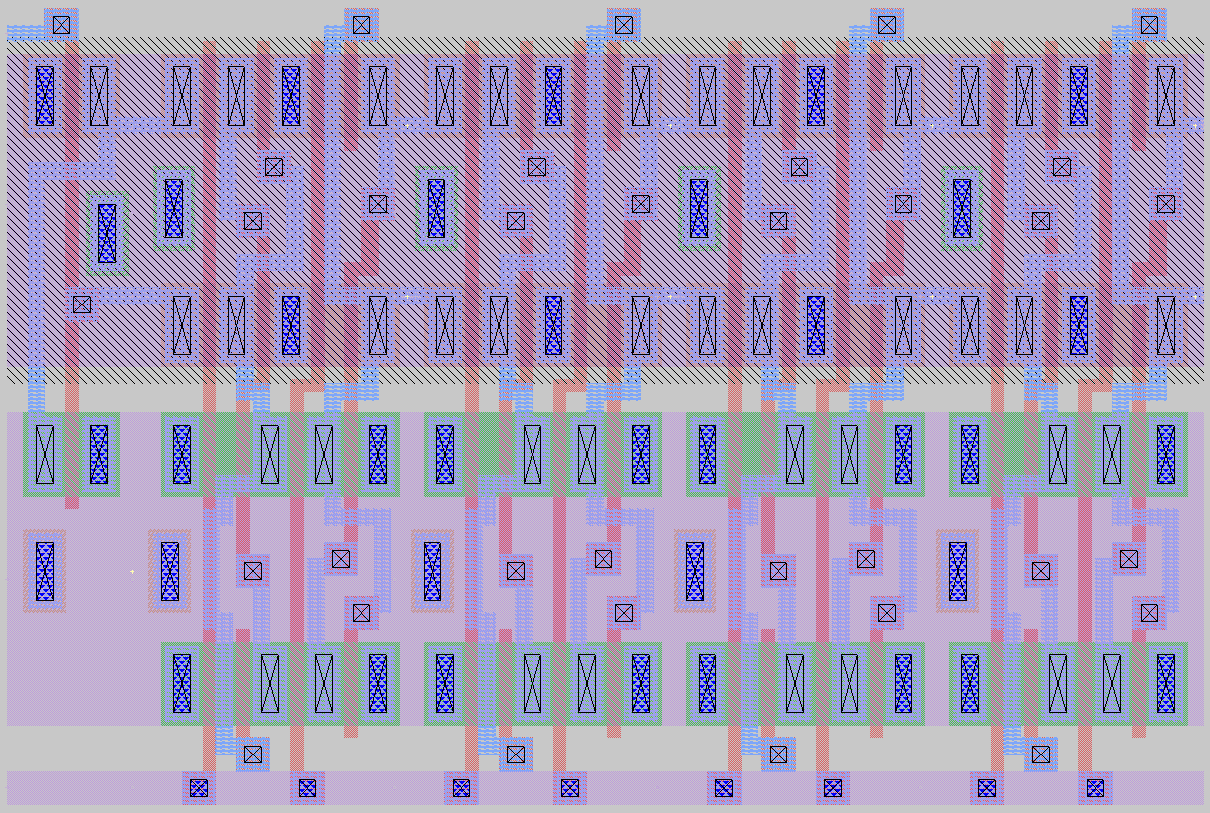
\includegraphics[width=0.8\linewidth]{../img/sreg_mag.png}
        \caption{\textit{Magic} layout of the shift register with inverter.}
        \label{fig:sregmag_inv}
    \end{figure}
    \FloatBarrier
    \section{Layout versus Schematic}
    Finally, I performed Layout-versus-Schematic comparison at all levels of the shift register. There are three listings below:
    \begin{enumerate}
        \item Layout versus Schematic for D Flip Flop
        \item Layout versus Schematic for Shift Register without Inverter
        \item Layout versus Schematic for Shift Register with Inverter
    \end{enumerate}
    \begin{lstlisting}[language=tcl, caption=\textbf{Layout versus Schematic for D Flip Flop}]
Equate elements:  no current cell.
Equate elements:  no current cell.

Subcircuit summary:
Circuit 1: layout/dff_lvs.spice            |Circuit 2: schem/dff_lvs.spice             
-------------------------------------------|-------------------------------------------
sky130_fd_pr__pfet_01v8 (8)                |sky130_fd_pr__pfet_01v8 (8)                
sky130_fd_pr__nfet_01v8 (8)                |sky130_fd_pr__nfet_01v8 (8)                
Number of devices: 16                      |Number of devices: 16                      
Number of nets: 13                         |Number of nets: 13                         
---------------------------------------------------------------------------------------
Resolving automorphisms by property value.
Resolving automorphisms by pin name.
Netlists match uniquely.
Circuits match correctly.
Cells have no pins;  pin matching not needed.
Device classes layout/dff_lvs.spice and schem/dff_lvs.spice are equivalent.
Circuits match uniquely.
    \end{lstlisting}
\begin{lstlisting}[language=tcl, caption=\textbf{Layout versus Schematic for 4-bit Shift Register}]
Equate elements:  no current cell.
Equate elements:  no current cell.

Subcircuit summary:
Circuit 1: dff                             |Circuit 2: dff                             
-------------------------------------------|-------------------------------------------
sky130_fd_pr__pfet_01v8 (8)                |sky130_fd_pr__pfet_01v8 (8)                
sky130_fd_pr__nfet_01v8 (8)                |sky130_fd_pr__nfet_01v8 (8)                
Number of devices: 16                      |Number of devices: 16                      
Number of nets: 13                         |Number of nets: 13                         
---------------------------------------------------------------------------------------
Resolving automorphisms by property value.
Resolving automorphisms by pin name.
Netlists match uniquely.
Circuits match correctly.

Subcircuit pins:
Circuit 1: dff                             |Circuit 2: dff                             
-------------------------------------------|-------------------------------------------
nD                                         |nD                                         
D                                          |D                                          
CLK                                        |CLK                                        
VN                                         |GND **Mismatch**                           
VP                                         |VDD **Mismatch**                           
Q                                          |Q                                          
nQ                                         |nQ                                         
---------------------------------------------------------------------------------------
Cell pin lists are equivalent.
Device classes dff and dff are equivalent.

Subcircuit summary:
Circuit 1: layout/shiftreg_4_lvs.spice     |Circuit 2: schem/shiftreg_4_lvs.spice      
-------------------------------------------|-------------------------------------------
dff (4)                                    |dff (4)                                    
Number of devices: 4                       |Number of devices: 4                       
Number of nets: 13                         |Number of nets: 13                         
---------------------------------------------------------------------------------------
Circuits match uniquely.
Netlists match uniquely.
Cells have no pins;  pin matching not needed.
Device classes layout/shiftreg_4_lvs.spice and 
schem/shiftreg_4_lvs.spice are equivalent.
Circuits match uniquely.

\end{lstlisting}
    \begin{lstlisting}[language=tcl, caption=\textbf{Layout versus Schematic for 4-bit Shift Register with Inverter}]
Flattening unmatched subcell shiftreg_4 in circuit layout/sreg.spice 
(0)(1 instance)
Equate elements:  no current cell.
Equate elements:  no current cell.

Subcircuit summary:
Circuit 1: dff                             |Circuit 2: dff                             
-------------------------------------------|-------------------------------------------
sky130_fd_pr__pfet_01v8 (8)                |sky130_fd_pr__pfet_01v8 (8)                
sky130_fd_pr__nfet_01v8 (8)                |sky130_fd_pr__nfet_01v8 (8)                
Number of devices: 16                      |Number of devices: 16                      
Number of nets: 13                         |Number of nets: 13                         
---------------------------------------------------------------------------------------
Resolving automorphisms by property value.
Resolving automorphisms by pin name.
Netlists match uniquely.
Circuits match correctly.

Subcircuit pins:
Circuit 1: dff                             |Circuit 2: dff                             
-------------------------------------------|-------------------------------------------
nD                                         |nD                                         
D                                          |D                                          
CLK                                        |CLK                                        
VN                                         |GND **Mismatch**                           
VP                                         |VDD **Mismatch**                           
Q                                          |Q                                          
nQ                                         |nQ                                         
---------------------------------------------------------------------------------------
Cell pin lists are equivalent.
Device classes dff and dff are equivalent.

Cell inverter disconnected node: CLK

Subcircuit summary:
Circuit 1: inverter                        |Circuit 2: inverter                        
-------------------------------------------|-------------------------------------------
sky130_fd_pr__nfet_01v8 (1)                |sky130_fd_pr__nfet_01v8 (1)                
sky130_fd_pr__pfet_01v8 (1)                |sky130_fd_pr__pfet_01v8 (1)                
Number of devices: 2                       |Number of devices: 2                       
Number of nets: 4                          |Number of nets: 4                          
---------------------------------------------------------------------------------------
Circuits match uniquely.
Netlists match uniquely.

Subcircuit pins:
Circuit 1: inverter                        |Circuit 2: inverter                        
-------------------------------------------|-------------------------------------------
nD                                         |Y **Mismatch**                             
D                                          |A **Mismatch**                             
VP                                         |VP                                         
VN                                         |VN                                         
---------------------------------------------------------------------------------------
Cell pin lists are equivalent.
Device classes inverter and inverter are equivalent.

Subcircuit summary:
Circuit 1: layout/sreg.spice               |Circuit 2: schem/sreg_lvs.spice            
-------------------------------------------|-------------------------------------------
inverter (1)                               |inverter (1)                               
dff (4)                                    |dff (4)                                    
Number of devices: 5                       |Number of devices: 5                       
Number of nets: 13                         |Number of nets: 13                         
---------------------------------------------------------------------------------------
Circuits match uniquely.
Netlists match uniquely.
Cells have no pins;  pin matching not needed.
Device classes layout/sreg.spice and 
schem/sreg_lvs.spice are equivalent.
Circuits match uniquely.

    \end{lstlisting}
\end{document}
